\section{Scopo e strumentazione}
Scopo dell'esperienza è quello di misurare le caratteristiche di circuiti costituiti da un amplificatore operazionale.Si analizzano dapprima l'amplificatore invertente e non; se ne misurano guadagno in funzione della frequenza e dell'ampiezza dell'ingresso . Si passa poi allo studio del circuito integratore e derivatore tramite l'analisi dei plot di bode e dello sfasamento tra ingresso e uscita. E' stato usato l'oscilloscopio per la misura delle d.d.p oscillanti ed il multimetro per quelli continui. Si è poi usato un generatore d'onda per la produzione di segnali oscillanti ed un generatore di tensioni continue per alimentare l'OpAmp.

\section{Amplificatore invertente}
\begin{figure}[h]
	\centering
	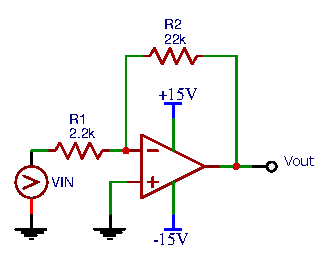
\includegraphics[scale=1]{opamp_invert.pdf}
	\caption{Amplificatore invertente.}
	\label{f:opamp_inv}
\end{figure}

Si è montanto il circuito in \fig{opamp_inv} e si è scelto $R_1= \SI{2.27(3)}{\kohm}$ e $R_2= \SI{22.1(3)}{\kohm}$ e la frequenza del generatore in ingresso è $f= \SI{1.0343(5)}{\kHz}$. Si è eseguito un fit lineare dei dati $V_{out} = aV{in}+b$. Si sono considerati solo i dati con $V_{in}<1.1$ V. I risultati del fit in \ref{f:guad_inv} sono :\\
$a= \SI{9.8(1)}{}$\\
$b= \SI{-0.02(4)}{}$\\
$\chi^2=4.70$ ($4$ dof, $p = 0.32$)\\
Provando a considerare anche i dati con $V_{in}$ superiore al cut-off si ottengono valori del $\chi^2$ con un p-value <0.15. Quindi supponiamo che tale cut-off sia la tensione limite oltre la quale si perde la linearità. Una verifica immediata si è fatta con l'oscilloscopio con $V_{in}=\SI{2.76(2)}{\V}$. Dalla \ref{f:clipping} si osserva un clipping del segnale in uscita chiaro segno della non linearità del circuito.
Il valore atteso del guadagno è $A= \frac{R_2}{R_1}= \SI{9.7(2)}{}$ che è compatibile con quello ottenuto dal fit.


\begin{figure}[h]
	\centering
	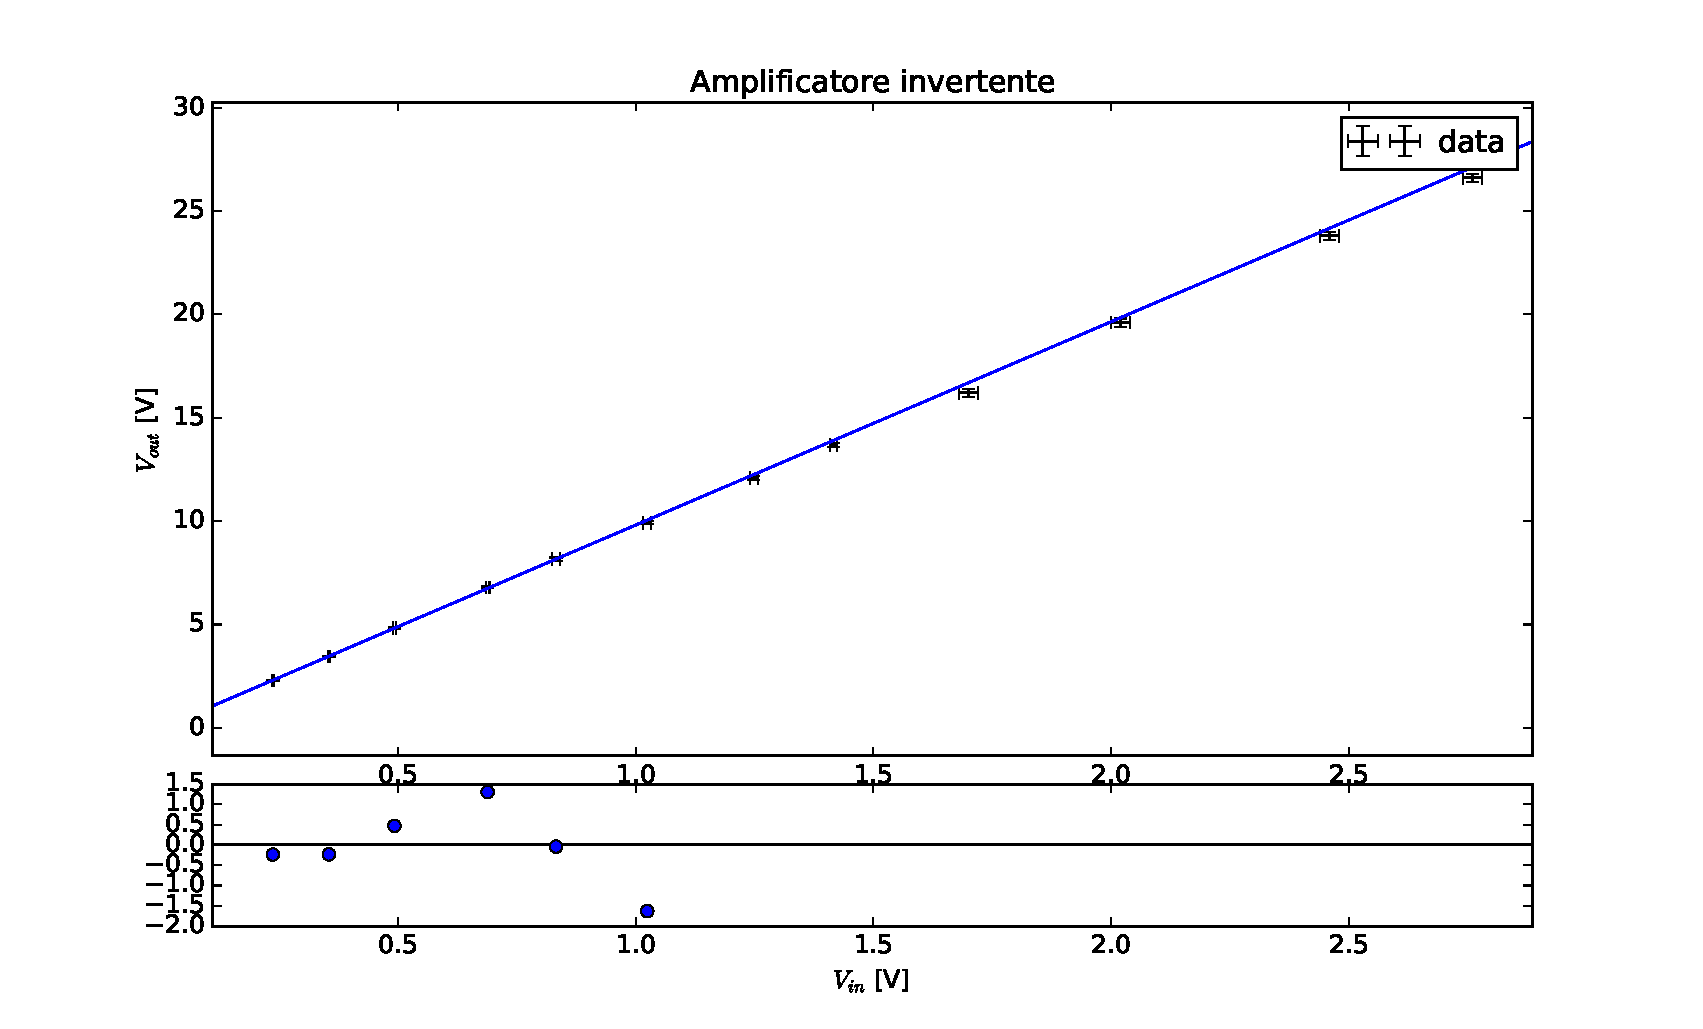
\includegraphics[scale=0.5]{fit_opamp_invertente.pdf}
	\caption{$V{out}$ in funzione di $V{in}$ per l'opamp invertente.}
	\label{f:guad_inv}
\end{figure}

\begin{figure}[h]
	\centering
	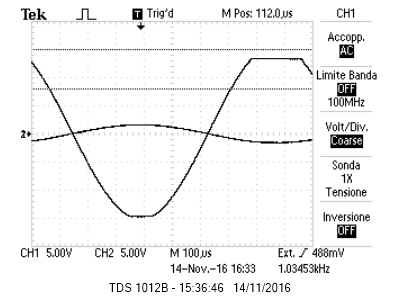
\includegraphics[scale=1]{clipping.png}
	\caption{Clipping di $V_{out}$ per l'opamp invertente.}
	\label{f:clipping}
\end{figure}

Si è poi misurata la resistenza di ingresso del'amplificatore inserendo in serie a $V_{in}$ una resistenza $R_s=\SI{2.27(3)}{\kohm}$ dello stesso ordine di grandezza di quella attesa.Poi è stato misurato $V_{out}$ con e senza $R_s$ inserita ottenendo rispettivamente $V_1=\SI{5.24(4)}{\V}$ e $V_2=\SI{10.32(8)}{\V}$. Da qui si ricava \\
$R_{ing}=\frac{R_sV_1}{V_2-V_1}= \SI{2.34(7)}{\kohm}$.\\
Tale valore è compatibile con quello atteso che è $R_1$.